\documentclass{beamer}
\usepackage[utf8]{inputenc}
\usepackage{palatino} % use palatino as the default font
\usepackage{listings}
\usetheme{Warsaw}

\lstset{ %
language=Octave,                % choose the language of the code
basicstyle=\tiny,       	% the size of the fonts that are used for the code
numbers=left,                   % where to put the line-numbers
numberstyle=\tiny,      	% the size of the fonts that are used for the line-numbers
stepnumber=1,                   % the step between two line-numbers. If it's 1 each line 
                                % will be numbered
numbersep=10pt,                  % how far the line-numbers are from the code
backgroundcolor=\color{white},  % choose the background color. You must add \usepackage{color}
showspaces=false,               % show spaces adding particular underscores
showstringspaces=false,         % underline spaces within strings
showtabs=false,                 % show tabs within strings adding particular underscores
frame=single,	                % adds a frame around the code
tabsize=2,	                % sets default tabsize to 2 spaces
captionpos=b,                   % sets the caption-position to bottom
breaklines=true,                % sets automatic line breaking
breakatwhitespace=false,        % sets if automatic breaks should only happen at whitespace
title=\tiny\lstname,            % show the filename of files included with \lstinputlisting;
                                % also try caption instead of title
escapeinside={\%*}{*)},         % if you want to add a comment within your code
morekeywords={*,...},           % if you want to add more keywords to the set
frameround=fttt,
}

\title{Analysing differences in tree data by Visual Analytics}
\author{Johannes Lichtenberger}\institute{Distributed Systems Group}

\begin{document}

\begin{frame}
\titlepage
\end{frame}

\begin{frame}
\frametitle{Application Domains}
\begin{itemize}
\item 
\end{itemize}
\end{frame}

\begin{frame}
\frametitle{Reasons}
\begin{block}{Why?}
Can you spot the differences of the two XML-files on the next slide?
\end{block}
\end{frame}

\begin{frame}[fragile]
\frametitle{Example}
\begin{lstlisting}[caption=first revision, frame=trBL]
<foo>
  <bar/>
  <baz>bla</baz>
  <foo></foo>hello bello<foo bla='blubb'/><do/>
  <jep>
    <klar></klar>
    super
    <blink/>
  </jep>
</foo>
\end{lstlisting}
\begin{lstlisting}[caption=second revision, frame=trBL]
<foo>
  <bar></bar>
  <baz>bl</baz>
  <foo></foo>hello bello<foo bla='bar'/><do/>
  <jep>
  <jep>
    <klar></klar>
    super
    <light/>
  </jep>
</foo>
\end{lstlisting}
\end{frame}

%\begin{frame}
%\frametitle{Challenges}
%\begin{block}{Preprocessing realworld data}
%Wikipedia, Network data, SVN data...
%\end{block}
%\begin{block}{Appropriate representation}
%Extended Sunburst view (Treering metapher), Treemap view (new layout algorithm)
%\end{block}
%\begin{block}{Being responsive}
%\begin{itemize}
%\item Treetank encoding
%\item Large data sets
%\end{itemize}
%\end{block}
%\end{frame}

%\begin{frame}
%\frametitle{Interaction}
%\begin{description}
%\item[Modifications] insert/delete/renames -- drag \& drop
%\item[Zooming/Panning] zoom in and pan out
%\item[Magnifier] Fisheye... 
%\end{description}
%\end{frame}

\begin{frame}
\frametitle{Challenges}
\begin{center}
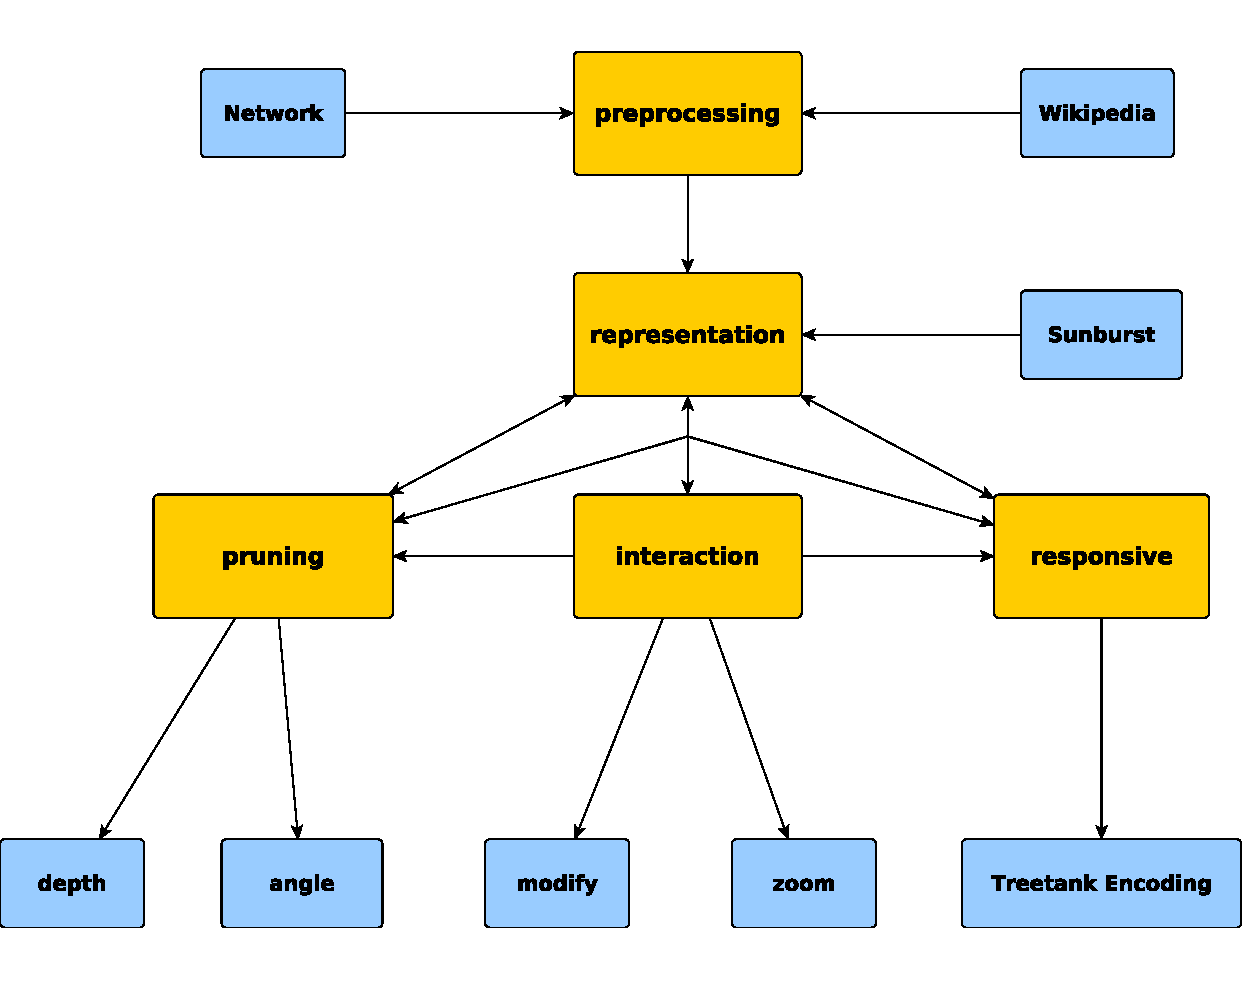
\includegraphics[height=3.0in]{images/challenges.pdf}
\end{center}
\end{frame}

\begin{frame}
\frametitle{GUI overview}
\begin{center}
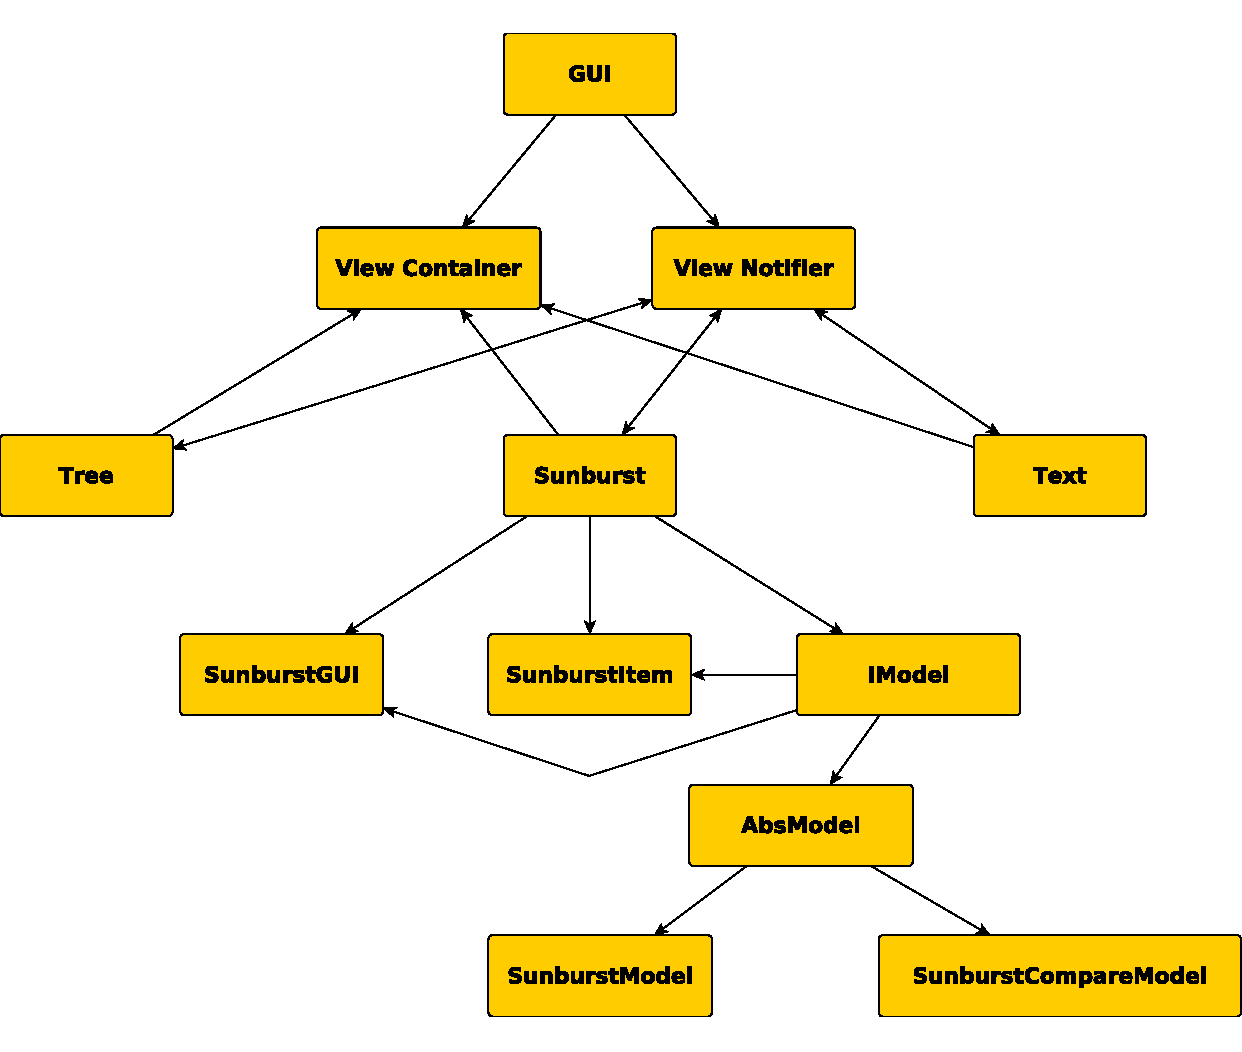
\includegraphics[height=3.0in]{images/overview.pdf}
\end{center}
\end{frame}

\begin{frame}
\frametitle{Screenshot}
%\begin{center}
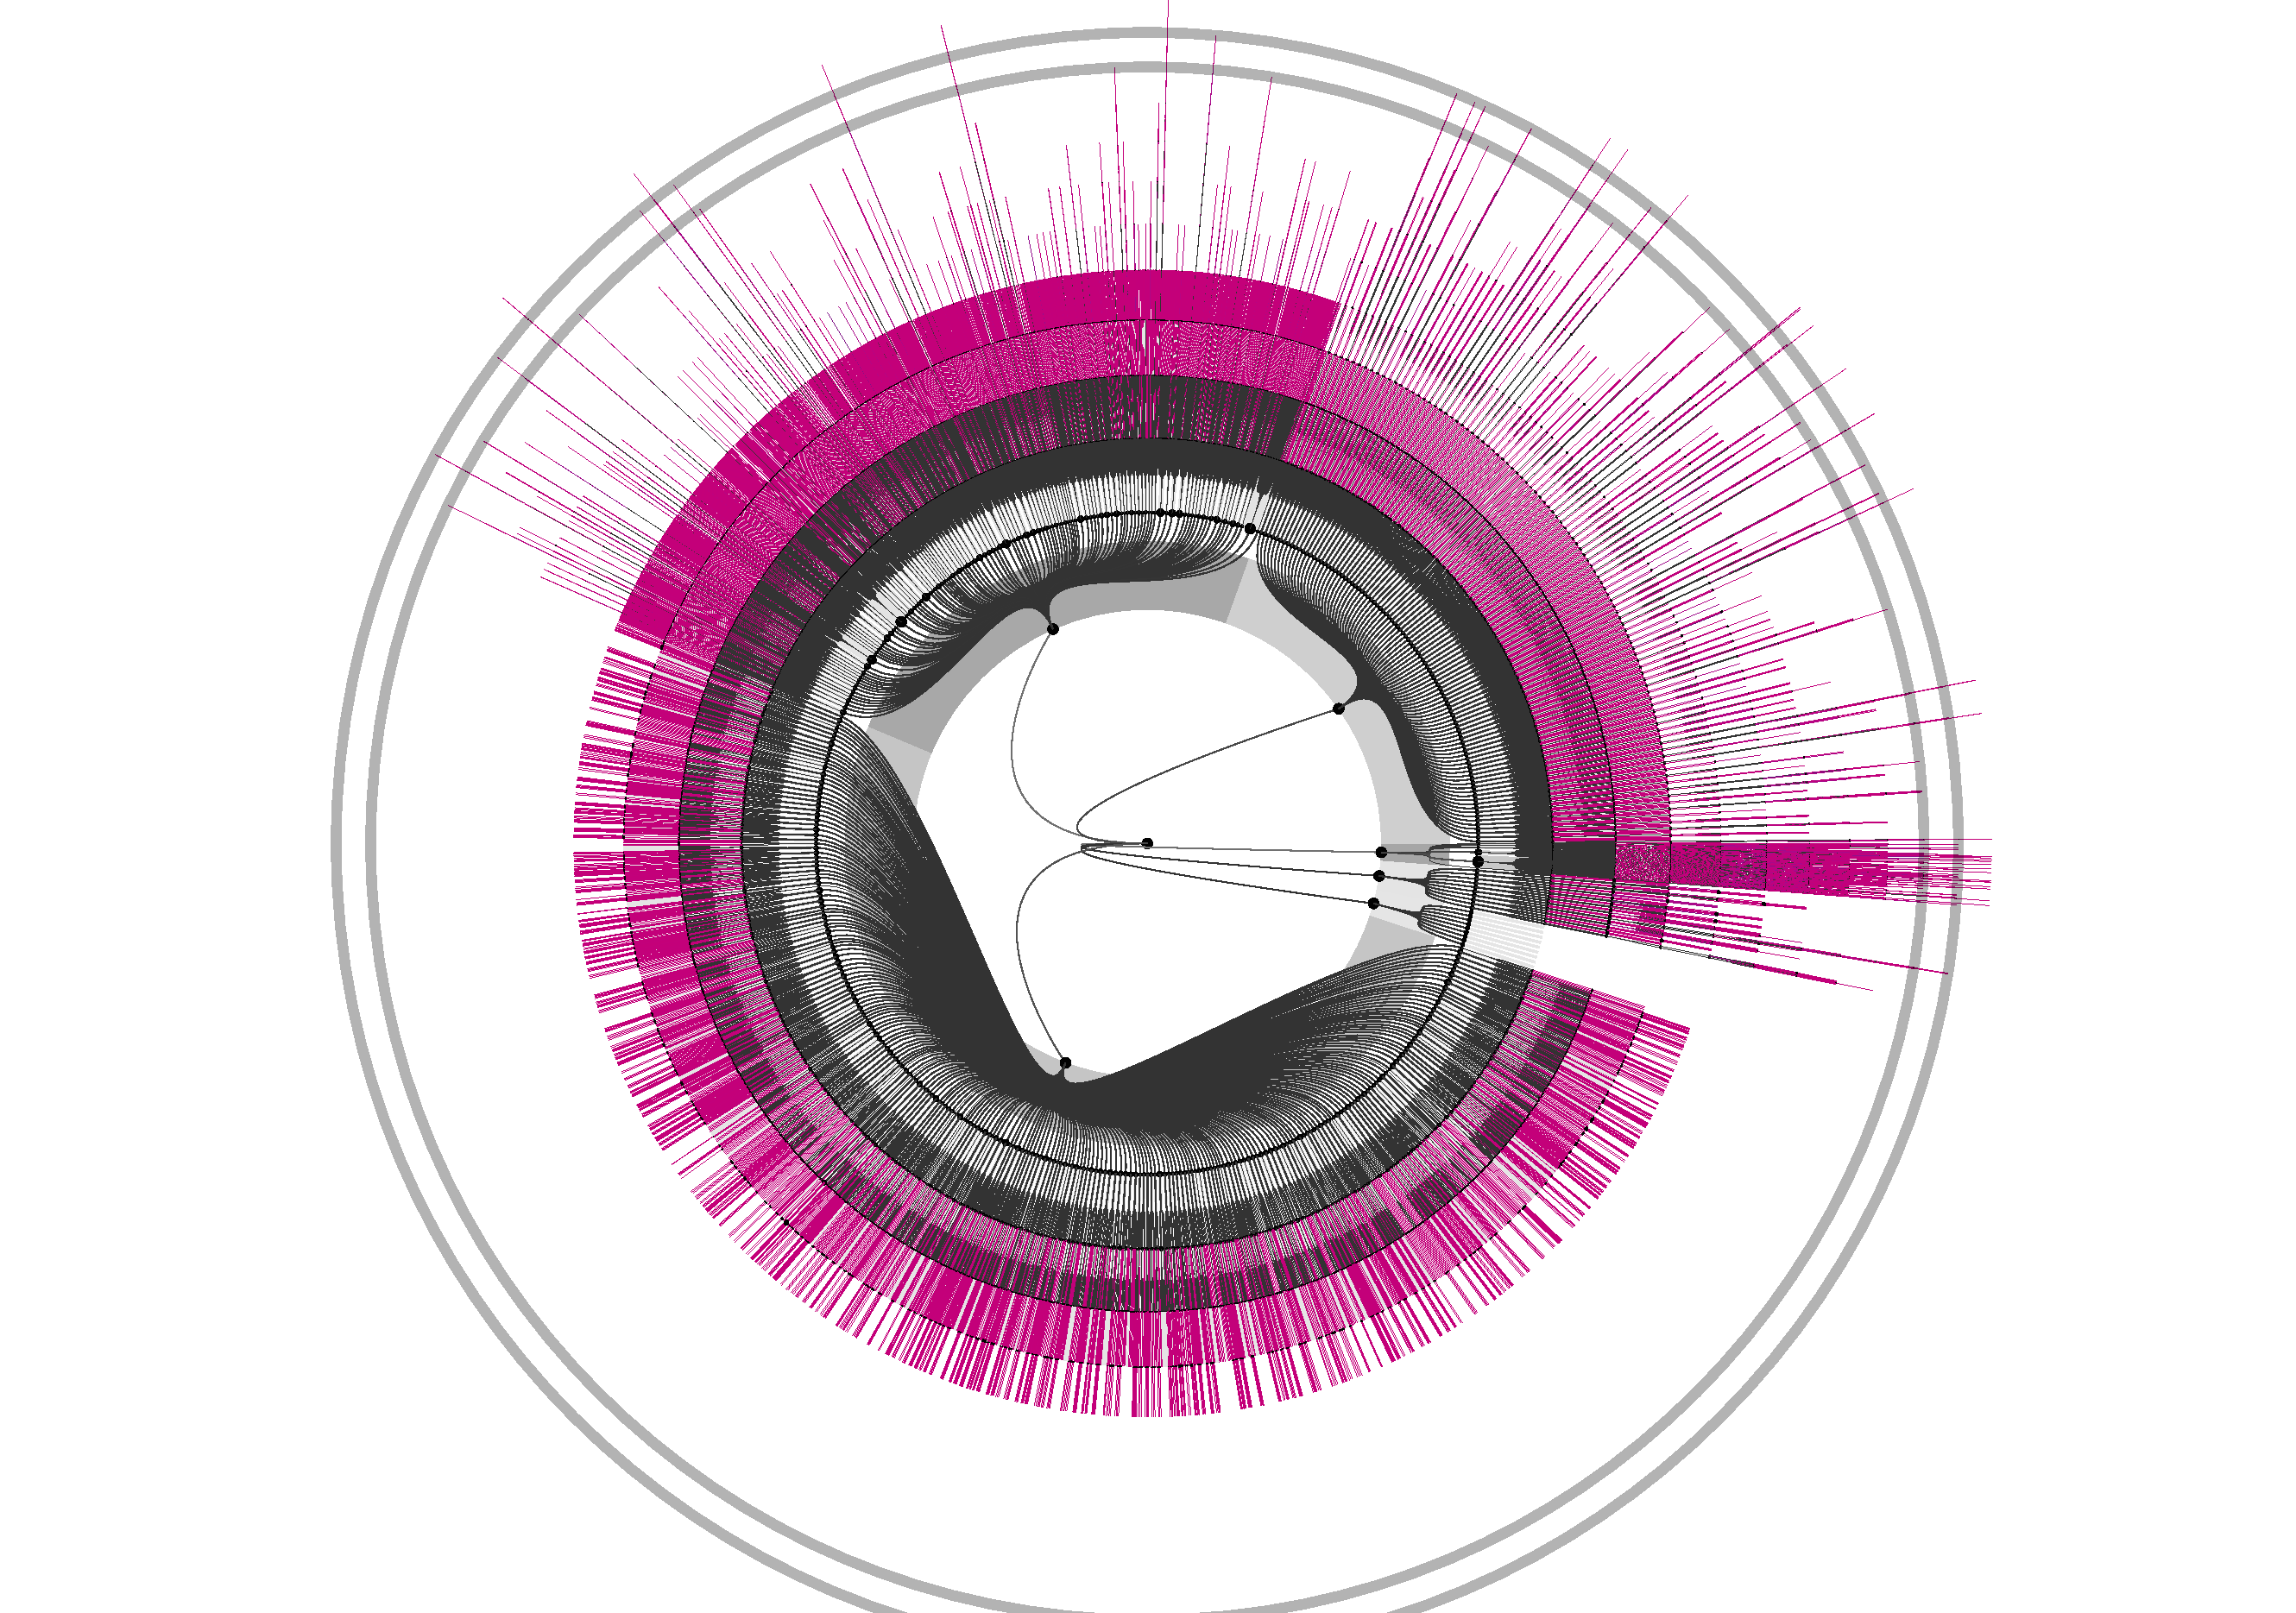
\includegraphics[height=3.0in]{images/101231_005715.pdf}
%\end{center}
\end{frame}

\begin{frame}
\frametitle{Screenshot}
%\begin{center}
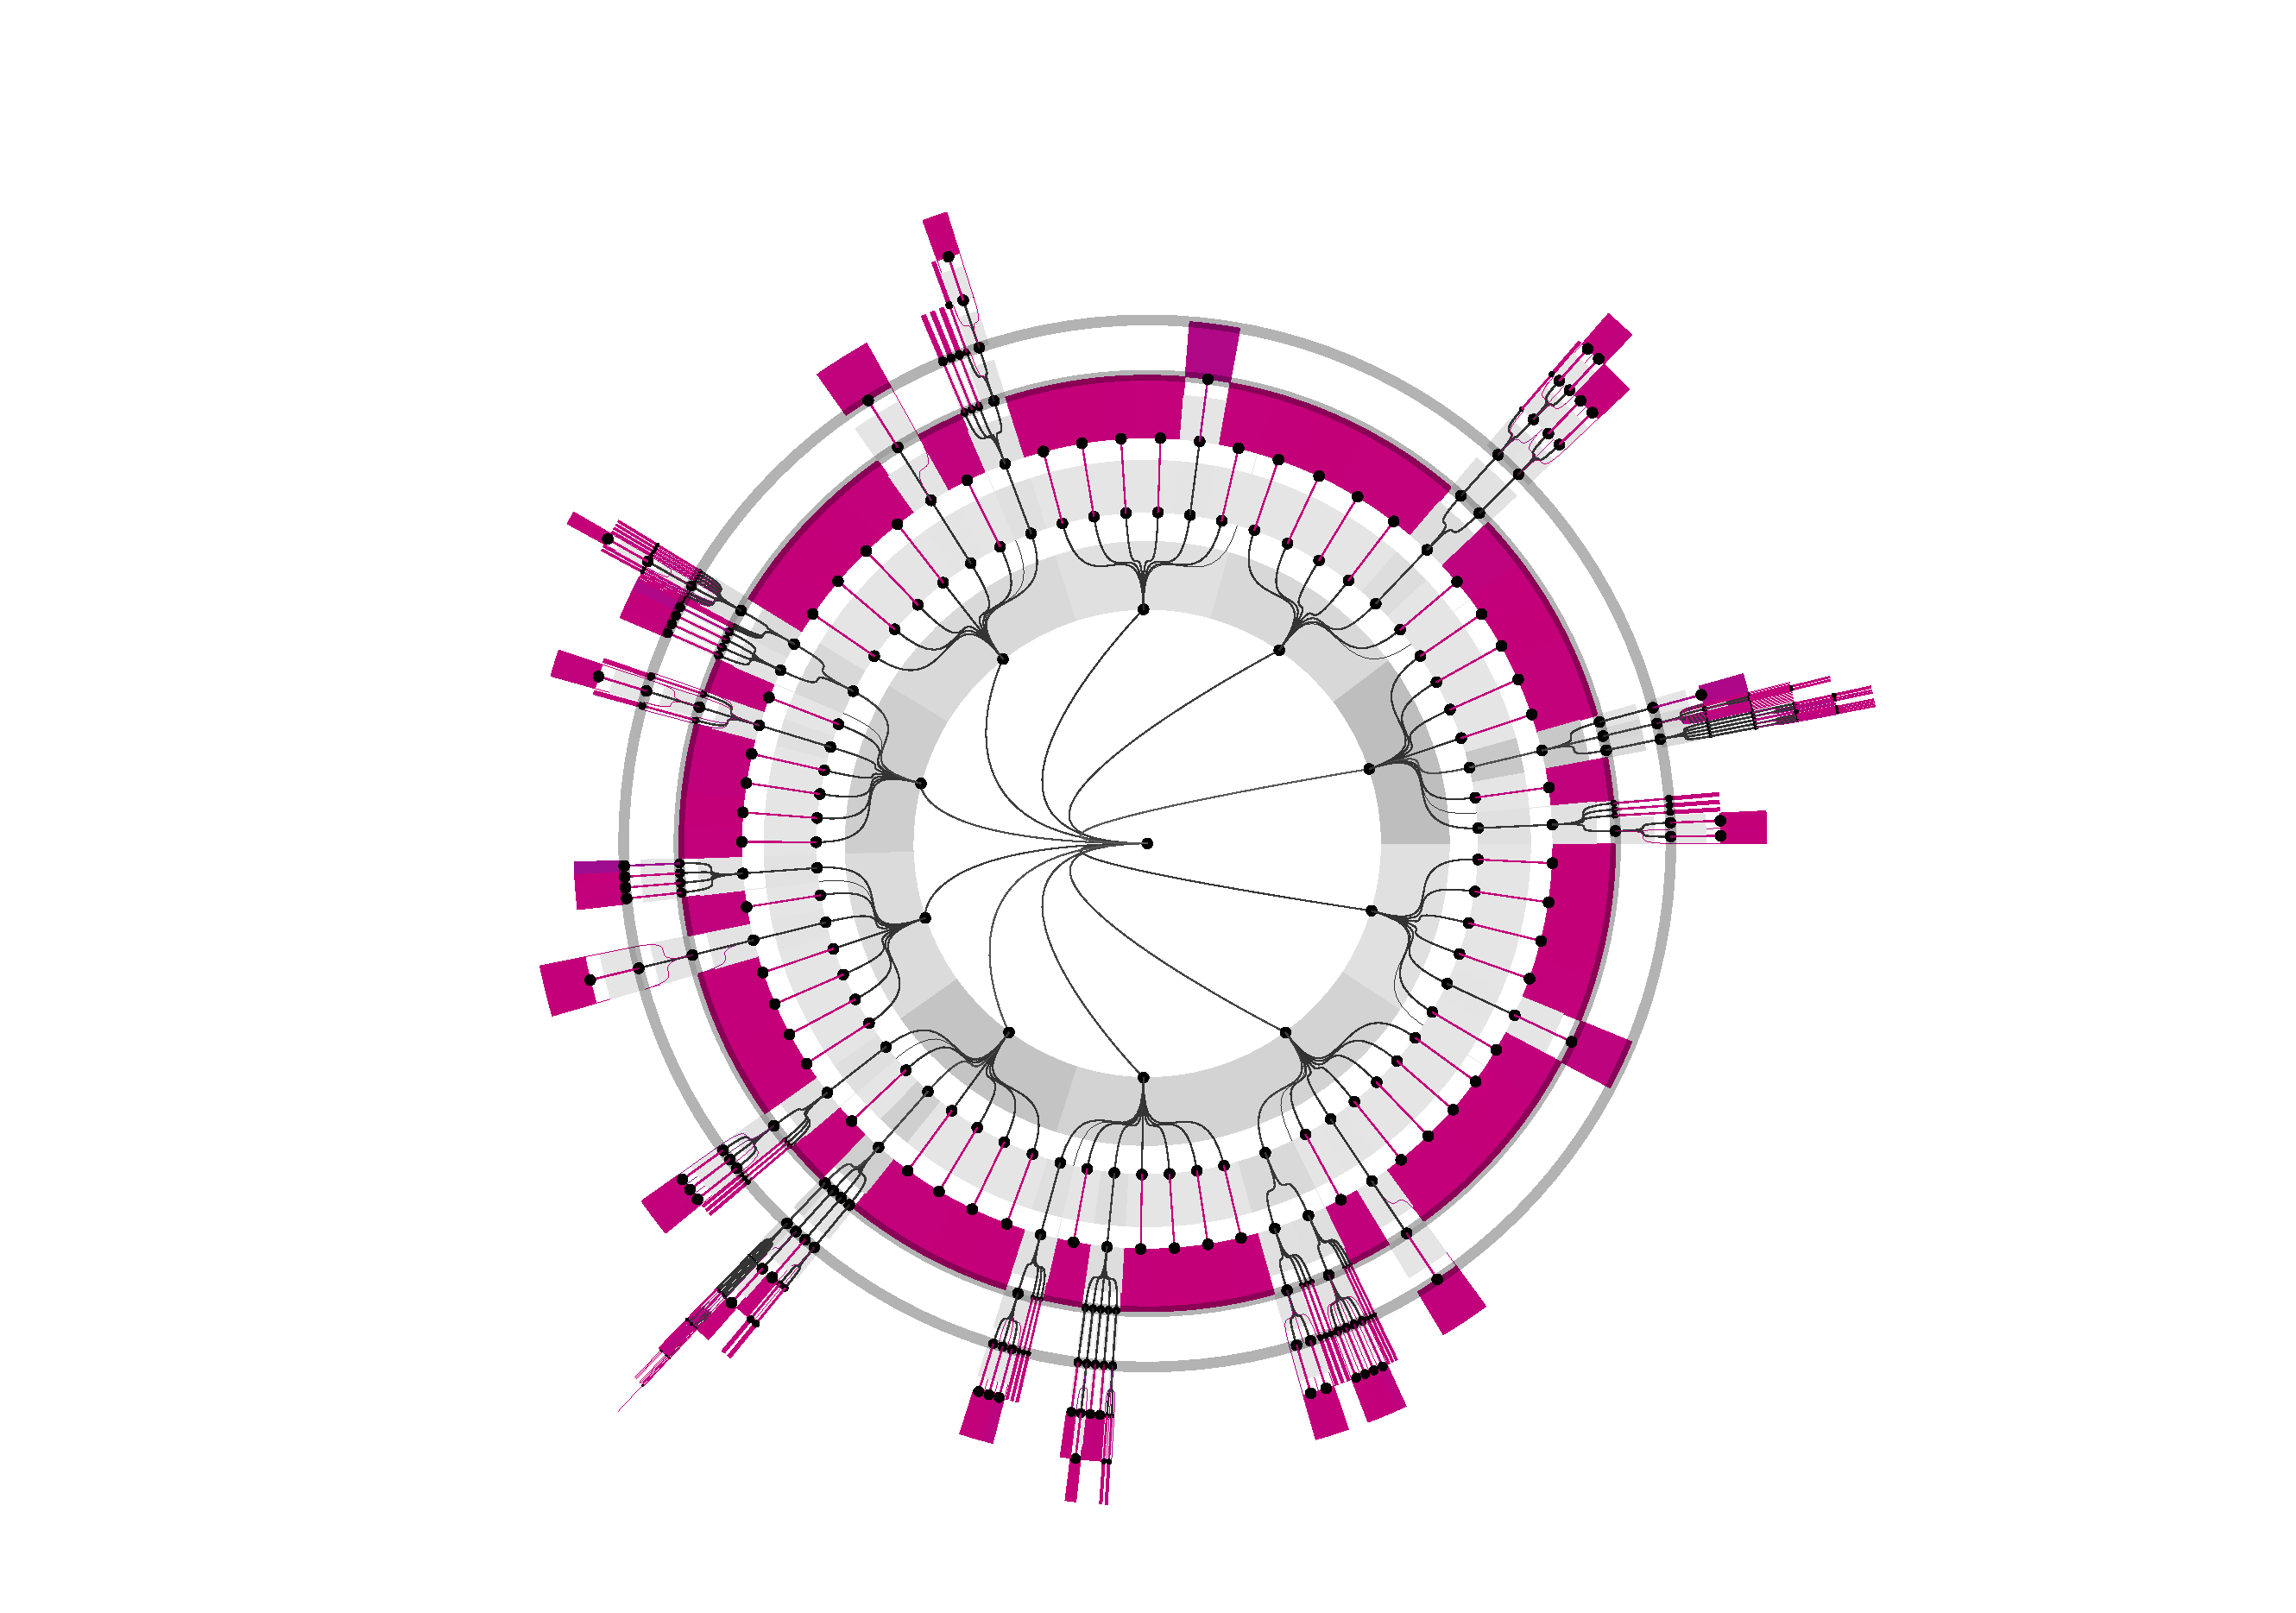
\includegraphics[height=3.0in]{images/101231_010038.pdf}
%\end{center}
\end{frame}

\begin{frame}
\frametitle{Demo}
Demo...
\end{frame}

\begin{frame}
\frametitle{Work to do}
\begin{itemize}
\item the diff view
\item inserting/deleting/renaming nodes
\item drag \& drop
\item working on the framework
\end{itemize}
\end{frame}

\end{document}
